\documentclass[12pt] {article}
\usepackage[margin=1in]{geometry} %one inch margins
\renewcommand{\baselinestretch}{1.5} %double space, safe for fancy headers
\usepackage{pslatex} %Times font
\usepackage{graphicx} %for figures
\usepackage{enumerate} %for lists
\usepackage{fancyhdr} %header
\pagestyle{fancy}
\usepackage[font={small,sf},format=plain,labelfont=bf,up]{caption}
\fancyhf{}
\fancyhead[l,lo]{150707V \textit{ Training Report}} %left top header
\fancyhead[r,ro]{\thepage} %right top header
\usepackage{kernelstyle}
\usepackage{listings}
\usepackage{amsmath,amssymb,amsfonts,amsthm}
\usepackage{graphicx}
% \usepackage[utf8]{inputenc}
\usepackage{float} 
\usepackage[caption=false,font=timesnewroman]{subfig}
\usepackage[final]{pdfpages}
\usepackage{gensymb}

\graphicspath{{figures/}}

\usepackage{xcolor}
\usepackage{soul}
\usepackage{hyperref}
\hypersetup{
    colorlinks=true,
    linkcolor=blue,
    filecolor=magenta,      
    urlcolor=cyan,
}
\captionsetup[figure]{labelfont={bf},name={Fig.},labelsep=period}
\captionsetup[table]{labelfont={bf},name={Table.},labelsep=period}
\usepackage{caption}
\usepackage{chngcntr} 
\counterwithin{figure}{section}
\counterwithin{table}{section}


\usepackage{algorithmic}
\usepackage[ruled, noend,lined,linesnumbered]{algorithm2e}

\newcommand{\hlc}[2][yellow]{{%
    \colorlet{foo}{#1}%
    \sethlcolor{foo}\hl{#2}}%
}

\usepackage{hyperref}
\hypersetup{
   colorlinks=true,
   linkcolor = black,
   citecolor=Green
}


\title{TRAINING REPORT}


\definecolor{hgray}{RGB}{130,130,130}
\definecolor{hred}{RGB}{136,0,0}
\definecolor{black}{RGB}{0,0,0}
\definecolor{Green}{RGB}{0,255,0}

\usepackage[T1]{fontenc}
\usepackage[tableposition=top]{caption}
\usepackage{rotating}
\usepackage{color, colortbl}
\usepackage{booktabs, array, dcolumn}
\usepackage{tikz}
\usepackage{graphicx}
\usepackage{pgf-umlsd}
\usepackage{multirow}
\usepackage{epsfig}
\usepackage{subfig}
\usepackage{pgfplotstable}
\usepackage{amsfonts}
\usepackage{relsize}
\usepackage{varwidth}
\usepackage{url}
\usepackage{amsmath}
\usepackage{amssymb}
\usepackage{booktabs}
% \usepackage{soul}
\usepackage[normalem]{ulem}
\usepackage{subfig}
\usepackage{kernelstyle}
\definecolor{Gray}{gray}{0.9}
\usepackage{hyperref}
% \usepackage{tabularx}
\usepackage{footnote}

\definecolor{gray1}{gray}{0.9}
\definecolor{gray2}{gray}{0.6}
\definecolor{Gray}{gray}{0.9}


\definecolor{light-gray1}{gray}{0.65}
\definecolor{light-gray2}{gray}{0.95}

%%------------------------ PREAMBLE ENDS ---------------------------

\begin{document}
\pagenumbering{roman} % Start roman numbering


\newpage

\tableofcontents
\newpage
\listoffigures
\listoftables
\newpage
\pagenumbering{arabic}
%!TEX root = ./intern_report.tex
\section*{Preface}

\paragraph{}
Described in this report is the 24 week training experience I had in wave computing/Paraqum Technologies dating from 25.06.2018 to 07.12.2018 for the fulfillment of industrial training requirements of my B.Sc. in Electronics and Telecommunication Engineering. The report consists of 3 main sections as follows

\subsubsection*{Chapter 1: Introduction to Wave computing and Paraqum Technologies}
\paragraph{}
Wave computing is a USA based AI startup and Paraqum Technologies is a Sri Lankan Electronic design startup. Wave is now ranked among the top 25 AI providers of the world~\cite{top25ai} and Paraqum Technologies is highly respected in Sri Lanka as a pioneer of the industry and recieves design contracts from all over the world. Our training was done through a design contract offered to Paraqum by Wave computing.

\subsubsection*{Chapter 2: Training Experience}
\paragraph{}
Even though I was an intern, I was given full exposure to the company workflow. I recieved a full scale project to lead and a support team from all over the world to work with. Everyone in the company were very supportive and friendly. The environment was comfortable to work and the workload was perfectly balanced, demanding yet not overwhelming.

\subsubsection*{Chapter 3: Conclusion}
\paragraph{}
I can say without a doubt, this is one of the best training experiences one can get. The University of Moratuwa Industrial training division, the Department of Electronic and Telecommunication Engineering and National Apprentice and Industrial Training Authority (NAITA) together did their best to provide us with an exceptional experience that will be very useful for the future of our careers.

\newpage
\section*{Acknowledgment}

\paragraph{}
I take this chance to show my gratitude towards everyone that helped make this training possible and facilitated my time with it. First of all I should thank the industrial training division of University of Moratuwa and the National Apprentice and Industrial Training Authority (NAITA) for allowing us to get an industrial training of this magnitude and quality during the time of our studies and always looking out for the wellbeing of the trainees.

\paragraph{}
I also would like to thank the administration and staff of Paraqum Technologies, starting with the CEO Dr. Ajith Pasqual, Manager Eng. Hasanka Sandujith, Eng. Kasun Tharaka who coordinated the internships and all other staff members who helped in a great many ways to make the training a staggering success. 

\paragraph{}
Last but definitely not least, The staff of the Wave computing team (later separated as Wave computing Sri Lanka) were always dedicated to make the training worthwhile for us. I sincerely thank the Senior Director of Software Engineering division of wave computing Eng. Henrik Esbenson, who visited and supervised us from time to time, General manager of Wave computing Eng. Nuwan Gajaweera, Technical leaders Eng. Upul Ekanayaka and Eng. Binu Amarathunga, My supervisors Eng. Achintha Ihalage, Eng. Omega Gamage and SDK team lead Eng. Dakila Serasinghe and all other staff members of wave computing for everything they did for us.

\vspace*{3cm}

\noindent Chinthana Wimalasuriya,\newline
Undergraduate,\newline
Department of Electronics and Telecommunication Engineering,\newline
University of Moratuwa.

\newpage
\section{Introduction to the Training Establishment}
%!TEX root = ./intern_report.tex

\subsection{Company Overview}

\paragraph{}
Wave Computing is a USA Silicon Valley based company that specializes in dataflow technology~\cite{waveintro}, an alternative to the tensorflow~\cite{tflow} technology used by tech giants such as {Nvidia} and {Google} to accelerate {AI} and neural net training. Although the company is relatively new to the game, they have had a number of notable achievements, which are explained below in detail. They outsource their design contracts to teams around the globe and one of these contracts was undertaken by Paraqum Technologies. This particular team works with the Software development kit ({SDK}) and the applications of the Wave dataflow platform.
\begin{figure}[h]
    \centering
    
\includegraphics[trim=0cm 0cm 0cm 0cm, clip=true,scale=1]{figures/wave_logo.png}
    \caption{Wave Computing logo\label{Fig:Wave}}\vspace{-4mm}
    \end{figure}


\paragraph{}
Paraqum Technologies is one of the very first truly Sri Lankan Electronics industry companies in the country. It undertakes Electronic design contracts from big companies from around the world such as Osprey video and of course, Wave Computing. They also have their own network product line. The company had one of their teams working on a design project of Wave Computing which split up in November 2018 to form the Sri Lankan branch of Wave Computing (pvt) Ltd. 
\begin{figure}[h]
    \centering
    
\includegraphics[trim=0cm 0cm 0cm 0cm, clip=true,scale=1]{figures/pqm_logo.png}
    \caption{Paraqum Technologies logo\label{Fig:Paraqum}}\vspace{-4mm}
    \end{figure}

\paragraph{}
My work was focused on the SDK layer of the Wave dataflow platform. This describes a large toolchain of software utilities that are the primary way that an advanced user would interact with the system. This team is also one of the busiest teams of the whole organization because of the sheer complexity of the SDK. In the context of the Sri Lankan staff, the SDK team is the heart of the whole project.


\subsection{Company History - Wave Computing}

\paragraph{}
Wave computing is primarily a project-turned-to-startup by Dr. Derek Meyer, who is also the current CEO. The idea is to design a processor to process the huge amount of data required for complex operations such as large matrix multiplication applications in parellel. He realized his idea in to a semiconductor manufacturing company, wave semiconductor, which has become a legacy as some urls of the company still reads wavesemi. As the prospect of Artificial intelligence became popular, the company understood that their time and effort is best invested in that field and hence, wave semiconductor reformed into Wave Computing AI.

\paragraph{}
To meet the demand for Artificial intelligence applications, wave computing has planned a series of devices which can fit the requirement of the users whether it is a large datacenter or a small scale business or mobile/{IoT} devices.
\begin{figure}[h]
    \centering
    
\includegraphics[trim=0cm 0cm 0cm 0cm, clip=true,scale=0.5]{figures/wave_server.png}
    \caption{Wave Datacenter Server Unit\label{Fig:waveserver}}\vspace{-4mm}
    \end{figure}

\begin{figure}[h]
    \centering
    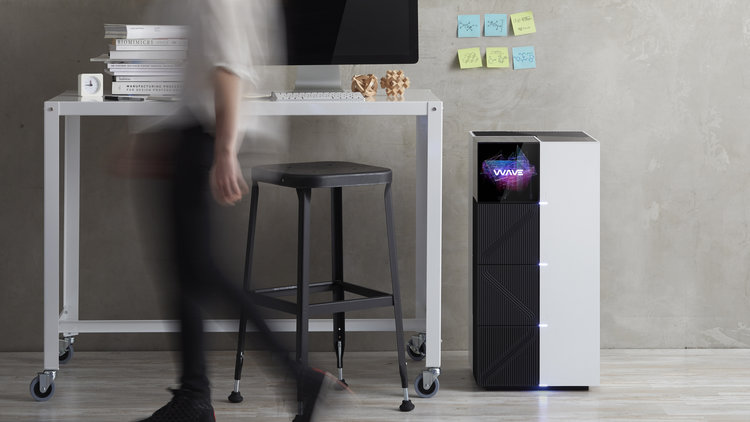
\includegraphics[trim=0cm 0cm 0cm 0cm, clip=true,scale=1]{figures/wave_lab.jpg}
    \caption{Wave Consumer Unit\label{Fig:wavelab}}\vspace{-4mm}
    \end{figure}

\subsection{Company}

\subsection{Organization Structure and Hierarchy}

\paragraph{}
CSIRO is divided into divisions, such as DATA61, Mining3, Energy and Health. DATA61 has a CEO: Adrian Turner and is divided further into groups: Robotics and automation systems (RAG), distributed sensor networks, data privacy group and so on. The employees can be categorized into staff (research engineers, PhD students), students (interns) and other staff. Multiple projects are done in RAG at the same time, and interns and PhD students work under a supervisor. Students can meet their supervisors at any time and there are weekly and monthly meetings between groups and divisions for further coordination.

\begin{figure}[h]
    \centering
    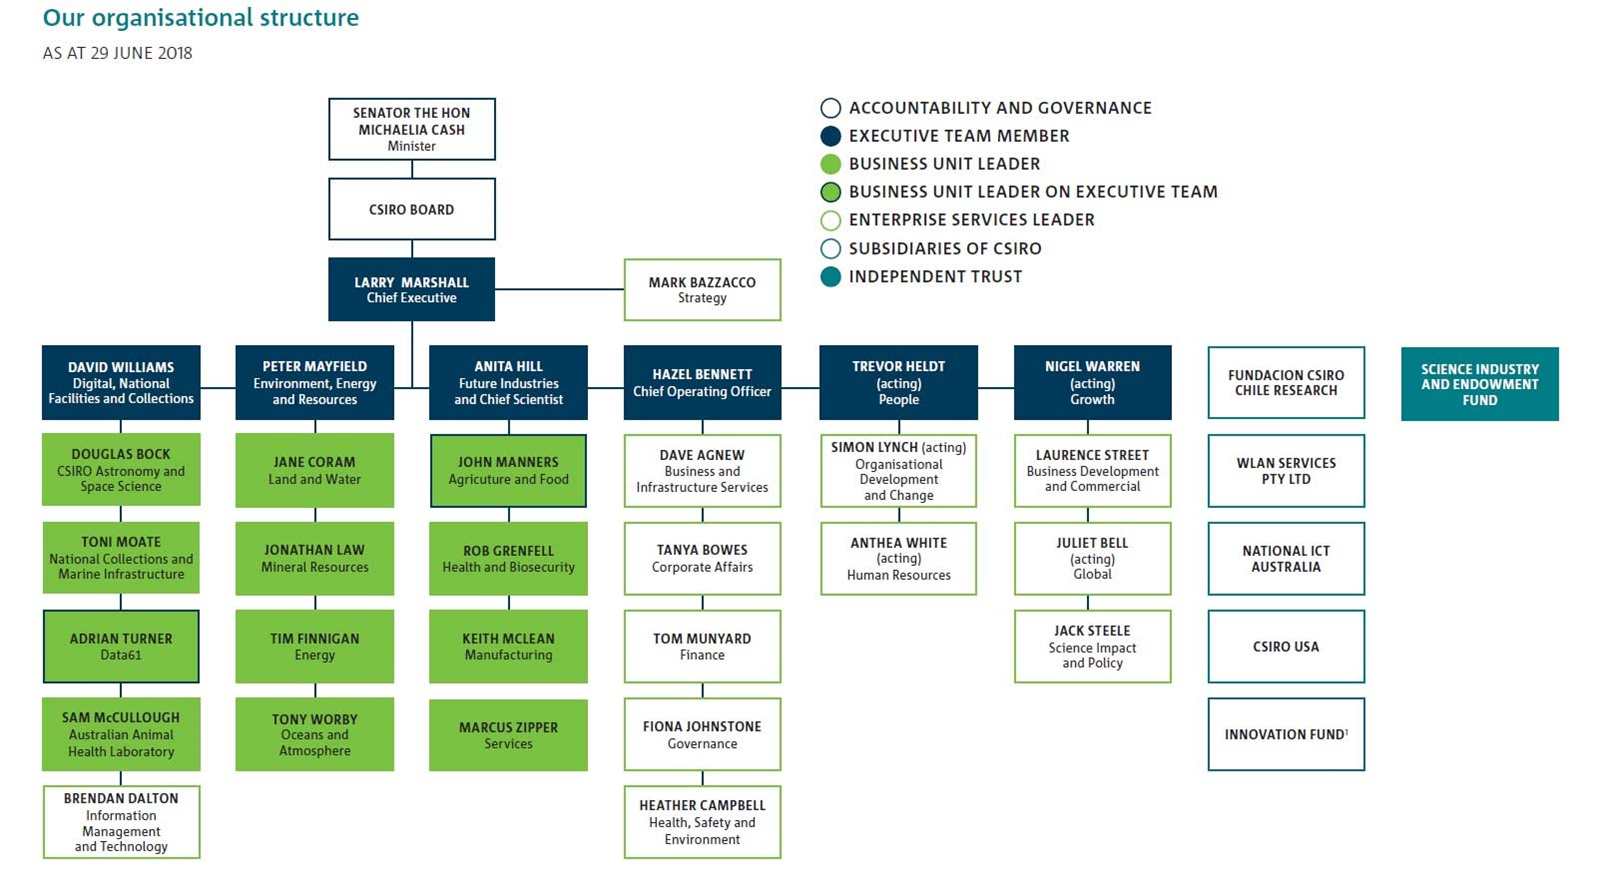
\includegraphics[width=16cm]{figures/csiro_struct.jpg}
    \caption{CSIRO Organizational Structure}\vspace{-4mm}
\end{figure}

\subsection{Areas of Interest}

\paragraph{}
DATA61 strives to build Australia's data driven future. Their programs can be divided into Analytics, Cyber-Physical Systems, Consumer Data Standards, Decision Sciences, Software and Computation Systems and Engineering and User Experience Design. Some of their key projects are:

\subsubsection*{Emesent - Hovermap}
\paragraph{}
Emesent is a spin-off company from the highly successful Hovermap project of DATA61. It is a state-of-the-art LiDAR based SLAM system to be fixed on industrial drones. Hovermap is also industrially used to analyze the structure and composition of various mineral deposits in rock cliffs, map underground mines and caves and used in forensics to analyze crime scenes.

\subsubsection*{SLAM}
\paragraph{}
DATA61 is a world leader in research, commercialization and impact of 3D LiDAR based simultaneous localization and mapping (3D SLAM). Their 3D SLAM algorithms and software is used to create highly accurate 3D maps of natural and artificial indoor and outdoor environments. This has been industrially used by the Australian Police to record homicide crime scenes, mapping caves, dinosaur footprints, record fragile cultural heritage sites and so on.

\subsubsection*{Legged Robots}
\paragraph{}
They have been focusing on Legged Robots since 2012. Modelled after insects, these six-legged and eight-legged robots can be used to navigate a disaster site and save lives. Several algorithms are being developed to address problems in legged navigation in complex environments.


\subsection{DARPA Subterranean Challenge}
\label{ssec:darpa}
\paragraph{}
The RAG of CSIRO was recently selected as one of the six funded teams worldwide for the DARPA Subterranean Challenge \cite{darpa} by United States Department of Defense. Therefore the next four years of research in Robotics in CSIRO will be more focused on developing robots that can simultaneously map and navigate complex environments such as underground tunnels, caves and mines without GPS or reliable communication with humans. It is an ideal project for DATA61, where their experience and expertise in SLAM, Hovermap and legged robots come together. By investing in this project for the next few years, DATA61 aims to develop new technology that can be later commercialized into different applications. 

%Image: Darpa challenge
\begin{figure}[H]
    \centering
    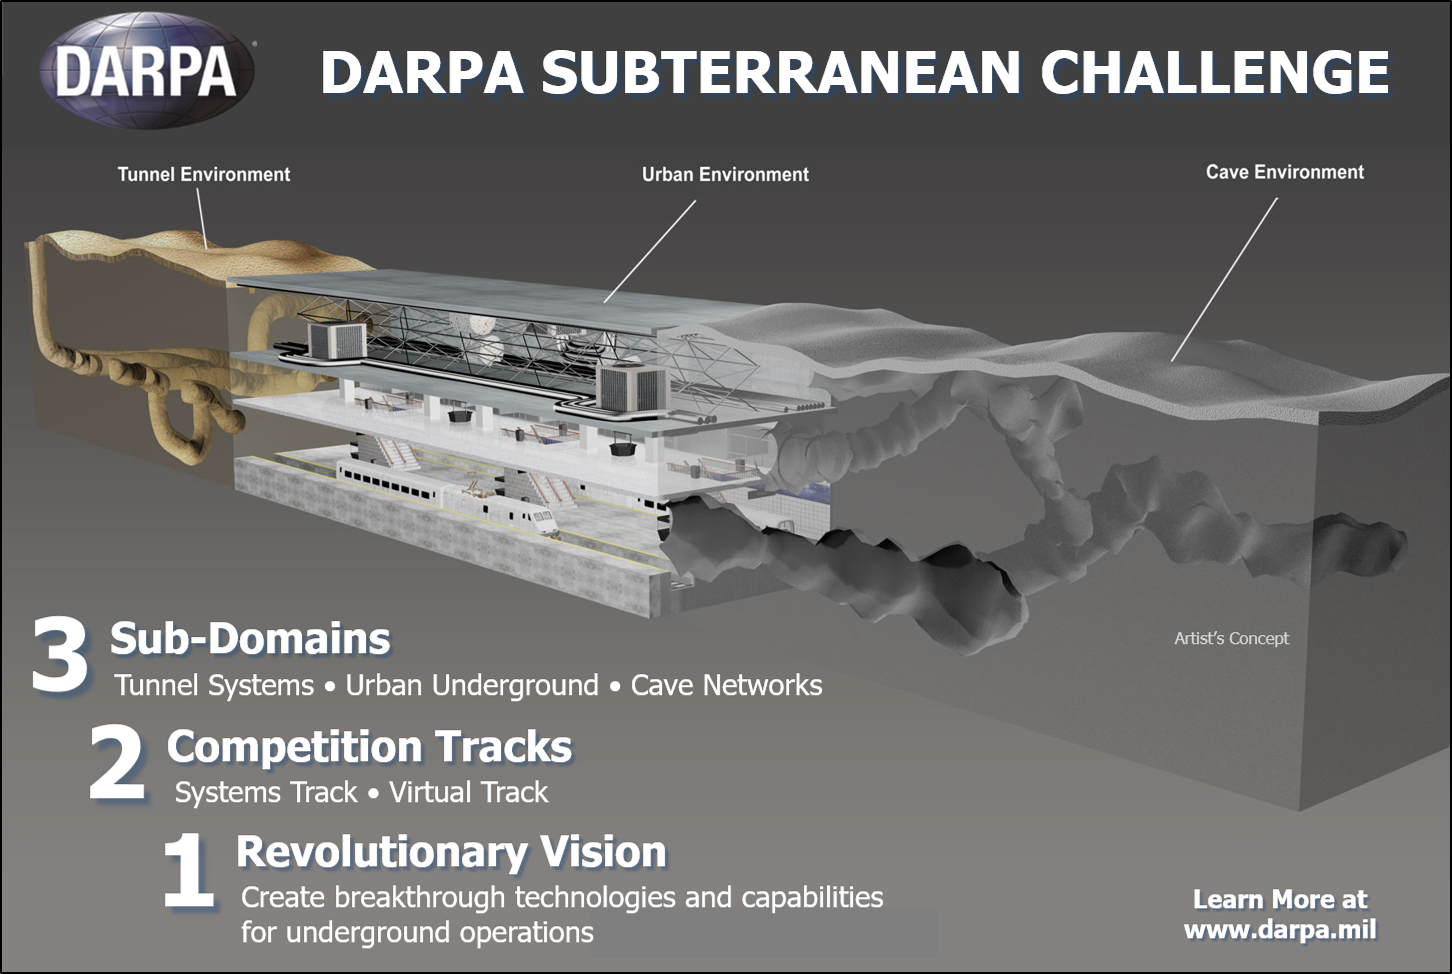
\includegraphics
        [width=12cm]
        {figures/subt_challenge.png}
    \caption{CSIRO focuses on DARPA challenge}\vspace{-4mm}
\end{figure}

\paragraph{}
This is the second competition held by DARPA to encourage development of cutting edge technology around the world. The first DARPA Robotics Challenge was held from 2012-2015 where the goal was to build a robot that can navigate a disaster site and perform tasks like driving a car, opening a door, drilling into the wall and so on, with an unreliable communications connection with the controlling humans. In case of future disasters like Fukushima Nuclear disaster, where humans cannot approach the site due to radiation, such robots can be utilized. The second competition focuses on subterranean environment, with the goal of buildings robots that can navigate the drug trafficking, human trafficking tunnels and save people stuck in mines and underground caves.

\paragraph{}
For this task, incorporating machine learning into the workflow of algorithm development and testing is of paramount importance for all researches in RAG. I addressed this problem by developing an efficient end-to-end pipeline for this and demonstrating it through two projects.


\subsection{Current Situation}
\paragraph{}
After years of research, development and commercialization of projects, DATA61 has risen as a world leader in many of their technologies. Hundreds of papers have been published from DATA61 in the past and are being published into reputed journals. Currently, DATA61 is being restructured and some of the technologies developed there have evolved into successful startup companies.

\subsection{Impacts on Sri Lankan Industry}
\paragraph{}
Being a part of the national research institute of Australia, DATA61 does not directly contribute to the Sri Lankan industry. However the research that is published in public domain can be used by Sri Lankan companies for their research and development.

\newpage
\subsection{SWOT Analysis}

\subsubsection*{Strengths}
\paragraph{}
DATA61 has ample resources and funds for its research programs. As a result a multitude of projects are being executed. Also the work culture in CSIRO encourages cross pollination of ideas and creativity. Their inclusive policy allows students and researchers from all around the world to come together and share their expertise and experience.

\subsubsection*{Weaknesses}
\paragraph{}
Although almost all researchers are friendly and helpful to each other, due to the way projects are assigned and due to the management structure, most of them work alone on a project. This has led to fragmentation, where people working on similar projects are unable to cooperate better. This is now addressed through weekly group meetings for Robotics, Machine Learning and standardization of the workflow, hardware and software APIs used in different projects.


\subsubsection*{Opportunities}
\paragraph{}
Being recognized as the world leader in their technologies, DATA61 has the opportunities to collaborate with other world class research institutes such as NASA Jet Propulsion Laboratory and ETH. We had the chance to attend lectures and discussions done by researchers from these institutes during our internship period. Also, DATA61 attracts talent from around the world and from within Australia, which would help them in the future research.

\subsubsection*{Threats}
\paragraph{}
DATA61 is a research organization that is funded for research that empowers the Australian industries. However, in the meanwhile they need to invest in pure science research the outcomes of which cannot be known in advance. This balance of funding projects of pure and applied science is vital to the success of DATA61 as an organization. If most of its research does not produce marketable technology, DATA61 is in danger of being under-funded by the australian government, meanwhile focusing more into applied science is not a sustainable strategy. This issue was discussed on multiple meetings as a part of their restructuring process.


\subsection{Usefulness to the Country}
\paragraph{}
DATA61 and CSIRO are important pillars of the Australian economy and society. The technologies materialized in DATA61 have laid the foundations for many companies in their industry and several companies collaborate with DATA61, paying them to use their service. This creates a win-win equilibrium that is beneficial to all parts of the economy.

\paragraph{}
Also, their research in healthcare, data privacy and infrastructure has been helping the australian society for the past few years. Their research into livestock management using IOT is helping the agriculture-based economy of the Queensland state. Hovermap and their research in mining is used to find new mineral deposits and analyze their composition. DATA61 is also modelling and devising algorithms to control traffic in different cities of Australia. 

\subsection{Suggestions to Improve the Company}
\begin{itemize}
    \item Implement a better project management system for intern students.
    \item Assign supervisors and well-defined projects that are compatible with the skills of students.
    \item Set deadlines for the student interns and monitor the progress.
    \item Provide concessions for students who live far away, as the public transport is considerably expensive.
\end{itemize}

\newpage
\section{Training Experience}
%!TEX root = ./intern_report.tex

\subsection{How I got the Opportunity}

\paragraph{}
A long time before the industrial training selection, I had heard Paraqum Technologies was one of the best places to learn about the electronics industry in Sri Lanka and Its CEO, Dr. Ajith Pasqual had taught a module in the university that sparked an interest in me about the subject of silicon design. Therefore, when Paraqum Technologies was listed as an open CV company, I did not hesitate to submit a CV, which got selected by the company staff who then interviewed me thoroughly in their office and sometime later, informed me that I had been selected to the Wave Computing Division.

\paragraph{}
At the start of the Internship, I was placed under the supervision of Eng. Achintha Ihalage, an application engineer whose original task was to handle the timing and constraints of the DPU chip. He walked me through the basics of setting up the Wave Computing workspace, company work ethics and other needed technical skills. He also introduced us to the DPU hardware and other proprietary technologies by Wave. 

\paragraph{}
During the second week, Eng. Henrik Esbenson, who is in charge of the Sri Lankan team at Wave HQ visited the office and demonstrated his ideas for projects. One of these was the Python - Wave Flow Graph translator, also known as Py2WFG. I volunteered to take that project and Eng. Henrik allocated me the necessary resources of the company including support teams and software tools to carry on the project.

\paragraph{}
This project soon became popular among the crowd of wave computing and I developed it according to the requirements and feedback. The amount of work was rather large but I managed to complete the project and hand it over by the time Internship ended. This project will most likely be adopted by full time developers and expanded to probably replace the existing design flow.


%!TEX root = ./intern_report.tex

\newpage
\subsection{The Teal Architecture and Wave Flow Graph(WFG)}
\paragraph{}
Teal is essentially the best of both programmable logic platforms and Application Specific Integrated Circuits(ASIC) combines together to give out the best performance and power efficiencies. In fact both hardware and software designs can be transferred onto the Teal fabric. Basically, Teal can be broken down into smallest unit of a Processing Element(PE). This is a simple processing unit which can carry out 8 bit operations adhering to Reduced Instruction SET (RISC) architecture.

\subsubsection{DPU Architecture}
\paragraph{}
A Processing Element will inherit an 8 bit accumulator who in return is connected to its neighboring Processing Elements. It is evident that a combination of a large number of such Processing Elements achieve as much parallelism as witnessed in the computational design history of the world. This revolutionary design with extensively parallel computational ability is a completely ground-breaking approach to the existing technologies used in chips for parallelism. Incidentally, a combination of 16 Processing Elements make up for a Cluster and a combination of 64 Clusters form a Super-Cluster and 16 such Super-Clusters form a single Wave Dataflow Processing Unit. The projected design for this massively complex structure has now reached the taping out process an it will only be a matter of time before the first chip gets manufactured physically. Such a developed Processing Element is projected to have a speed of close to 10GHz.

\begin{figure}[h]
    \centering
    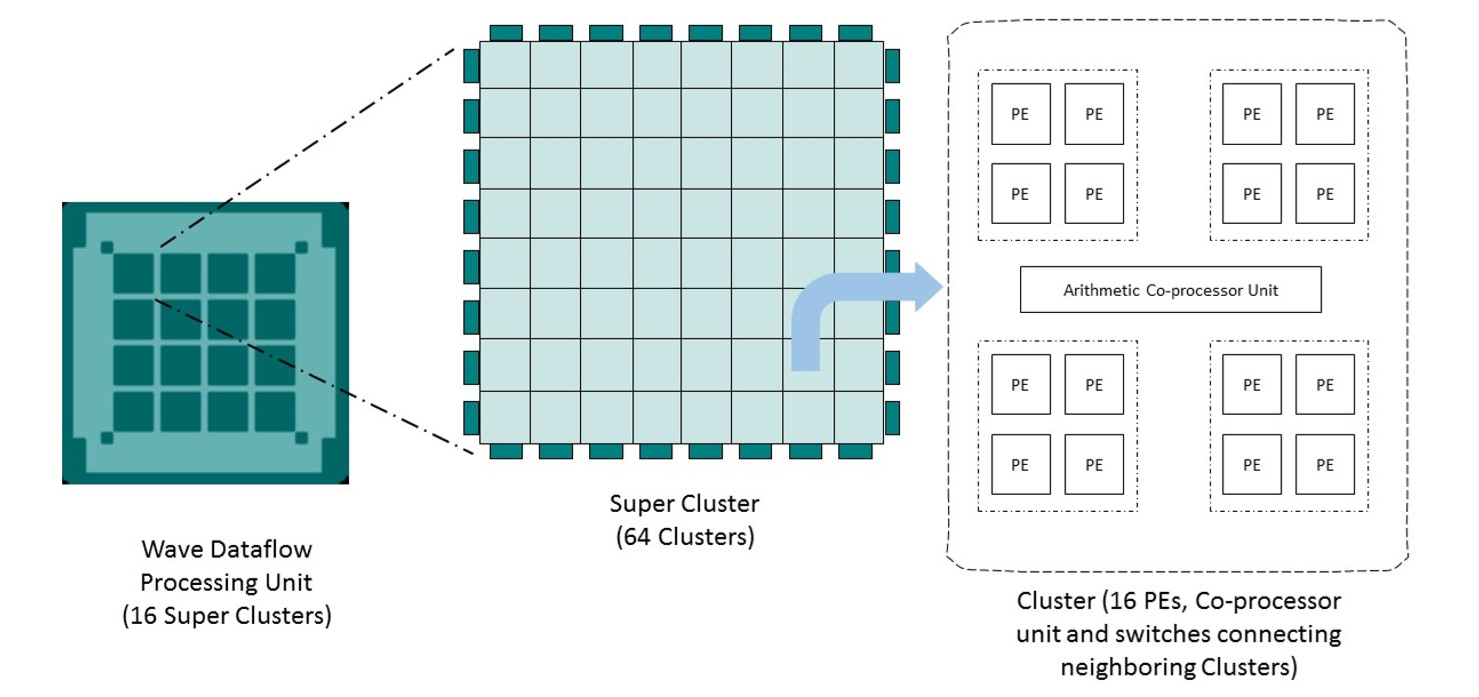
\includegraphics[trim=0cm 0cm 0cm 0cm, clip=true,scale=0.5]{figures/dpu_struct.jpg}
    \caption{Wave DPU with Processing Elements(PEs)\label{Fig:dpustruct}}\vspace{-4mm}
    \end{figure}

\paragraph{}
The Figure~\ref{Fig:dpustruct} is a comprehensive illustration of the structure of Teal design. It is noteworthy to realize that each Processing Element acts much similar to a single processing unit and therefore, each Super Cluster can be viewed in the perspective of thousands of processing units ready to function simultaneously. Nevertheless, the true power of Wave Dataflow Processing Unit design is shown in Figure~\ref{Fig:dpuboard} where the extent of operation of the final design is depicted. The final design is projected to have a whopping 2 Peta Operations per second amount of power which is ideally suited for the needs of computational power of the future. It is safe to say that Wave Dataflow Processing Unit will become by far the fastest ever processing unit of the world.

\begin{figure}[h]
    \centering
    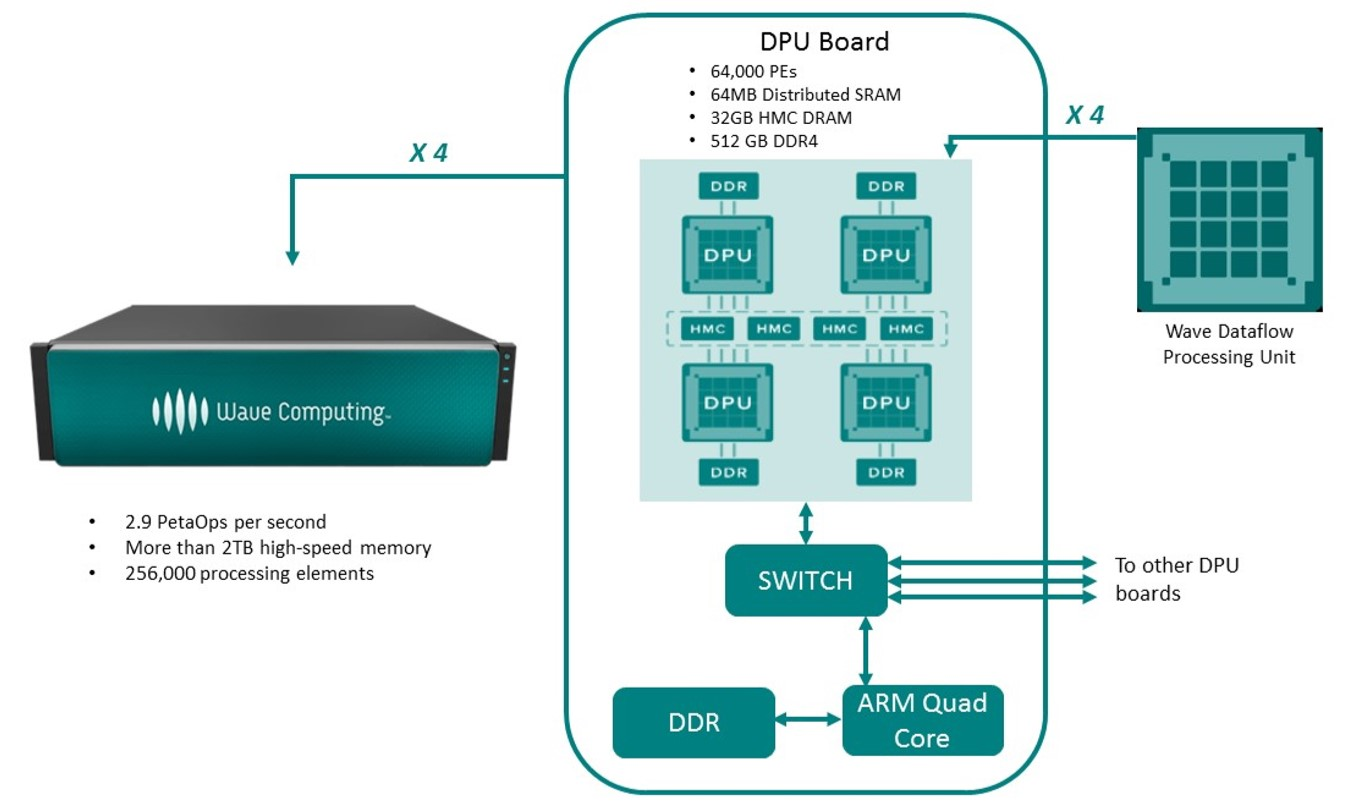
\includegraphics[trim=0cm 0cm 0cm 0cm, clip=true,scale=0.45]{figures/dpu_board.jpg}
    \caption{Wave Deep Learning Computer\label{Fig:dpuboard}}\vspace{-4mm}
    \end{figure}

\subsubsection{SoC Perspective}
\label{sec:socper}
\paragraph{}
The Teal processing accelerator is essentially integrated into a System-on-a-Chip(SoC). As shown in the Figure~\ref{Fig:socpers} it is connected to processor SoC using streaming AXI interfaces. It has a direct connection toward high speed IO streams. The DMA controller (refer Figure~\ref{Fig:socpers}) is the key connector between external DRAM internal Block RAMs of Teal. The accelerator itself is demand driven, meaning it will stay at sleep state unless instructed otherwise. The importance of this viewpoint was important to me as some of the design work carried out were finding a way to simulate DMA inputs and outputs. Since accessing data from external RAMs is through DMA ’Channels’, some of the work related to improvements in the DMA engine were carried out during my project executions. 

\paragraph{}
The next interesting design feature of Wave Data-flow processing model are the Wave Flow Graphs. This is a representation scheme for which operations are represented as nodes and values as edges. Nodes and edges connect together in a network of operations to perform a computational task. The idea behind the clock-less operation of the tasks come through the ability for nodes to perform the intended operation whenever valid inputs are provided. A dedicated clock is not needed and thus presence of valid data at the inputs automatically will define trusted operation. 

\paragraph{}
However, a sense of timing is available in the form of the concepts of tics and sub-tics. A tic is equivalent to a circular round of operations executed by a Processing Element buffer which is currently defined as 256 instructions. In fact, it is 256 times the instruction cycle time. Due to the fact that instruction cycle time is not specifically designated but rather dependent on the execution of each operations’ processing speed, it is not fair by the Wave DPU design to have a specific tic-rate. Incidentally, there is a typical rate of 10 GHz for a sub-tic cycle. a sub-tic cycle is essentially the rate at which an instruction from a circular buffer(IRAM) is fetched, processed and switched. 

\begin{figure}[h]
    \centering
    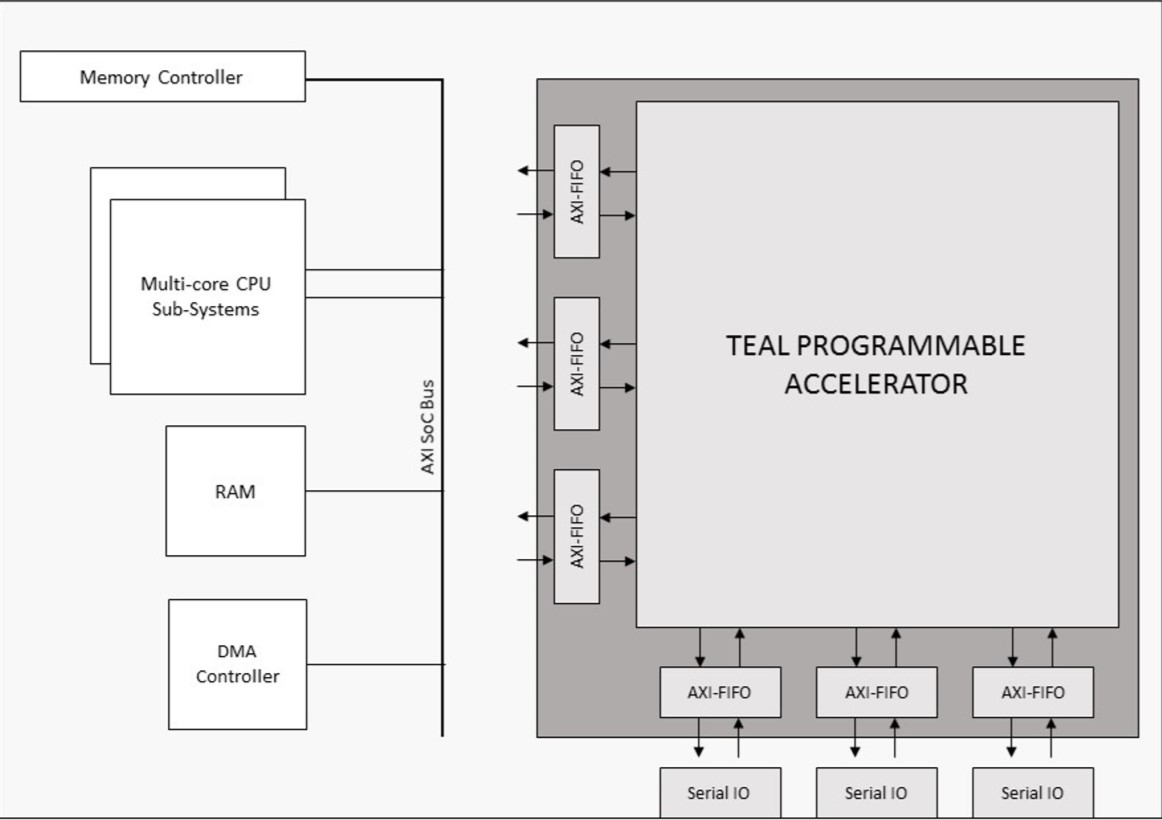
\includegraphics[trim=0cm 0cm 0cm 0cm, clip=true,scale=0.5]{figures/soc_pers.jpg}
    \caption{SoC Perspective of Teal Programmable Accelerator\label{Fig:socpers}}\vspace{-4mm}
    \end{figure}

\paragraph{}
Apart from the contrast between the parallelized implementation of Wave Flow Graph designs and the continuous flow of operations within PEs, Wave Flow Graph is a defined rule to represent any program within the Teal fabric. In XXXXXXX section 1.3.3 (Unit Testing) XXXXXX a direct implementation of testing the Wave Flow Graph operations carried out by me, is explained in detail.

\subsubsection{Wave design flow}
\paragraph{}
Owing to the complexity of parallel PE operation it is evidently clear that programming instructions into the Teal Architecture is not achievable manually. Therefore, an EDA flow is prevalent so that any hardware design can be brought down through compilation, scheduling, mapping and routing to the Teal fabric level. This flow of compilation from hardware design to Byte-fabric level is done through the Wave introduced design flow. The Figure~\ref{Fig:wfgstruct} is a representation of a very simple Wave Flow Graph design where you can see the nature of operation of the language. It basically consists of bit wise operations between inputs and outputs. Most operations are related to bit level manipulation of data and it is note worthy to realize that these operations are carried out for 8 bit data chunks. The combination of several bytes of data can be processed with special modules of Wave Flow Graph code where the data is subdivided and processed accordingly. The node edge representation of the design will give you enough ides as to the complexity that can arise with the introduction of several operations and variables into one design. The final structure will be a collection of various nets combined together from input end to output end.

\begin{figure}[h]
    \centering
    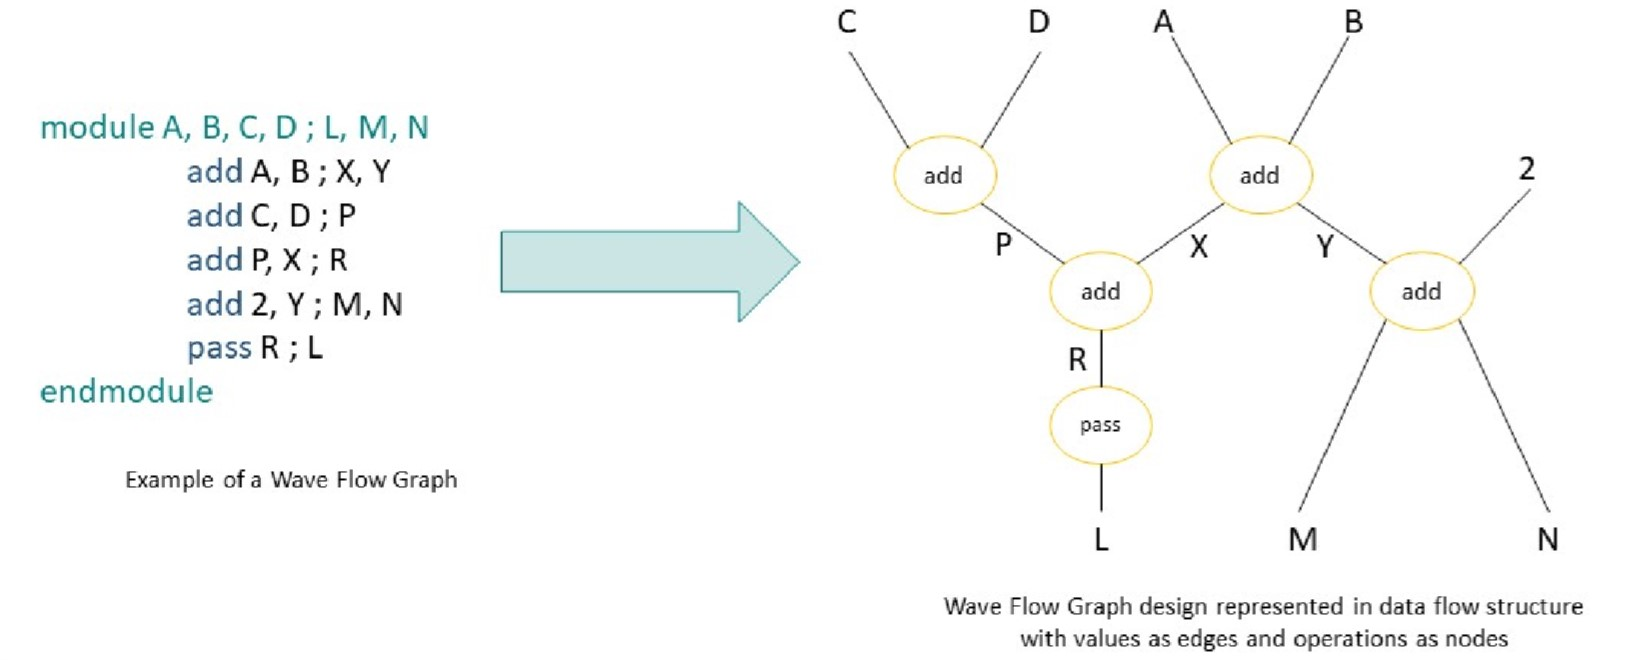
\includegraphics[trim=0cm 0cm 0cm 0cm, clip=true,scale=0.5]{figures/wfg_struct.jpg}
    \caption{Data flow structure of Wave Flow Graph designs\label{Fig:wfgstruct}}\vspace{-4mm}
    \end{figure}

\pagebreak
%!TEX root = ./intern_report.tex

\newpage
\subsection{Dive Framework and Wave toolchain}

\subsubsection{Framework Overview}

\paragraph{}
When writing a new design for the DPU, the engineers use an in-house written API called the dive framework for testing and Verification. Due to the sheer complexity of the programs that need to be adapted to run in the DPU, the code is brought down to lower semantic levels step by step using the toolchain which consists of 5 main tools.

\begin{itemize}
    \item Wave C Compiler (WCC) - Compiles the C++ code to a WFG code 
    \item Wave Flow Graph Simulator (WFGsim) - Simulates the flow graph and compares it with the I/O values of the C++ code
    \item Wave Flow Graph Compiler (WFGC) - Compiles the WFG code to a Wave Assembly code
    \item Wave Machine Simulator (WMsim) - Simulates the Wave assembly code in a virtual machine environment
    \item Wave Assembly Compiler (WAsm) - Compiles the assembly code to an encrypted binary file format called Lantana
\end{itemize}


\begin{figure}[h]
    \centering
    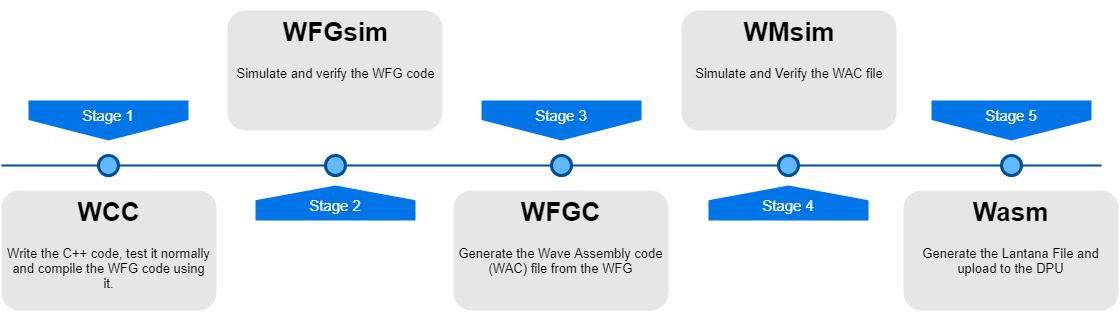
\includegraphics[trim=0cm 0cm 0cm 0cm, clip=true,scale=0.35]{figures/wave_flow.png}
    \caption{Wave Toolchain and design flow\label{Fig:waveflow}}\vspace{-4mm}
    \end{figure}

\subsubsection{Repository Structure}
\paragraph{}
Different cloud folders that contains software code are known as repositories. Wave source codes are stored in five main repositories hosted in a local git server. For better identification, the tools are again divided in to two classes, Wave Front End (WFE) and Wave Back End (WBE). WCC, WFGsim and WFGC belong to the WFE while WMsim and WAsm are contained in the WBE. In the Wave source code, the code for WFE and WBE are stored in separate repositories while the code that is shared by these are stored in a third repository named wcore. Test codes are stored in the wtest repository while experimental tools are stored in the final repository, tools.

\subsubsection{WCC}
\paragraph{}
Wave computing has their own version of C++ dubbed WaveC, which is C++ with added support for data channels and some more things. This language receives constant updates from a team inside wave and thus, developers must build the C language from its source code frequently. This is also true for other tools.

\paragraph{}
WCC uses a technology called LLVM~\cite{LLVM} to convert one human written code in to a different human readable code. It works by analyzing the code and simplifying it to a desired level and assembling the result back together on a predefined syntax. After simplifying the code again and again, the desired output can be obtained, which in this case is the WFG code file.

\subsubsection{WFGsim}
\paragraph{}
This was the most important tool for me since my project could eventually evolve to fully replace this tool. I had to analyze this tool very thoroughly to extract functionality for the Py2WFG simulator (section \ref{sec:py2wfgsim}). 

\paragraph{}
WFGsim works by multi-thread programming on python. It initializes separate threads for DPU sections and host processors. Inside each python thread, a library called boost is used to invoke a linear C++ script. These scripts 'talk' to each other via the python interface and python interface also gives the DPU sections a sense of time by governing the order which operations are executed.
%!TEX root = ./intern_report.tex

\newpage
\subsection{Py2WFG: A better way to write Wave Flow Graph}
\subsubsection{Python Vs. WFG}

\begin{figure}[h]
    \centering
    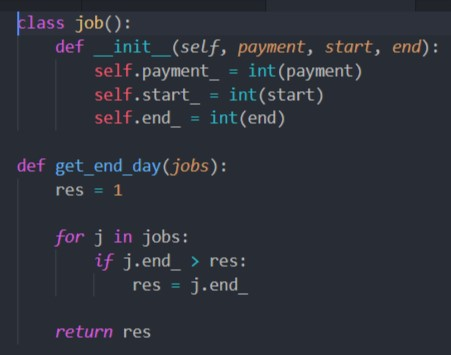
\includegraphics[trim=0cm 0cm 0cm 0cm, clip=true,scale=0.8]{figures/py_eg.jpg}
    \caption{Typical Python code snippet\label{Fig:pyeg}}\vspace{-4mm}
    \end{figure}

\paragraph{}
The Figure~\ref{Fig:pyeg} shows a typical python code example and Figure~\ref{Fig:wfgstruct} shows a WFG snippet. These two languages were built for two entirely different purposes but the highly adaptable nature of python makes a valid point whether if it can replace the functionality of WFG. But both languages have their pros and cons.

\subsubsection*{Python}
\paragraph{}
Python is a general purpose scripting language which focuses on user friendliness. It supports object oriented programming and is also backed up by a huge number of highly optimized libraries for various purposes. But when compared with languages such as C++ and Java, Python is heavy on the memory and slow for large volume computing. It is also not optimized for the particular purpose of programming the Wave DPU.

\subsubsection*{WFG}
\paragraph{}
WFG was created with one purpose and one purpose only in mind, Programming the Wave DPU. Thus it has primary operators that can precisely match the deep capabilities of the DPU hardware. It can be very efficient too when properly programmed. The downside to this language is that it is very strongly typed and is a user friendliness nightmare. Repetitive operators need to be manually entered by the user and the language has no capability of any kind of looping of the language itself.

\subsubsection{Python to WFG translator(Py2WFG)}
\paragraph{}
A solution was created by putting the best of both worlds together. The idea is to create a python 'sleeve' to cover up the WFG interface and present the user with a way to interact with python and get WFG level results. The user will now write up the script and when he runs it, it will output a fully optimized WFG script. 

\begin{figure}[h]
    \centering
    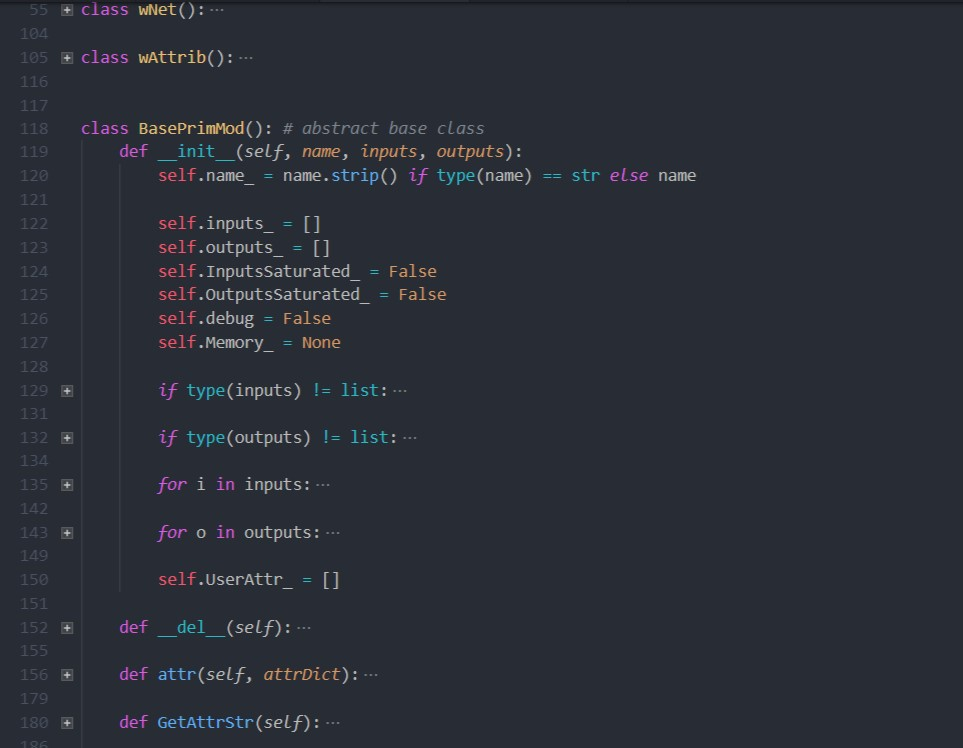
\includegraphics[trim=0cm 0cm 0cm 0cm, clip=true,scale=0.6]{figures/py2wfg_src.jpg}
    \caption{Part of the Py2WFG source code\label{Fig:py2src}}\vspace{-4mm}
    \end{figure}

\subsubsection*{Code Translation}
\paragraph{}
The basic idea for this library is derived from Tensorflow~\cite{tflow}, which is a python library that allows easy neural net design using a python library. The user will still need a sufficient knowledge on WFG syntax to use the library. But it will eliminate the hassles of writing a slightly-above-assembly language scripts by hand. The script that user needs to write is similar to the one showed in Figure~\ref{Fig:py2eg}. The library needs to be imported in to the script, Then Modules can be created from the wMod class in the library. These module 'husks' are then filled with dataflow operations as needed. When complete, issuing the makeWFG command will write a full WFG script that can be later integrated into the existing wave design flow.

\begin{figure}[h]
    \centering
    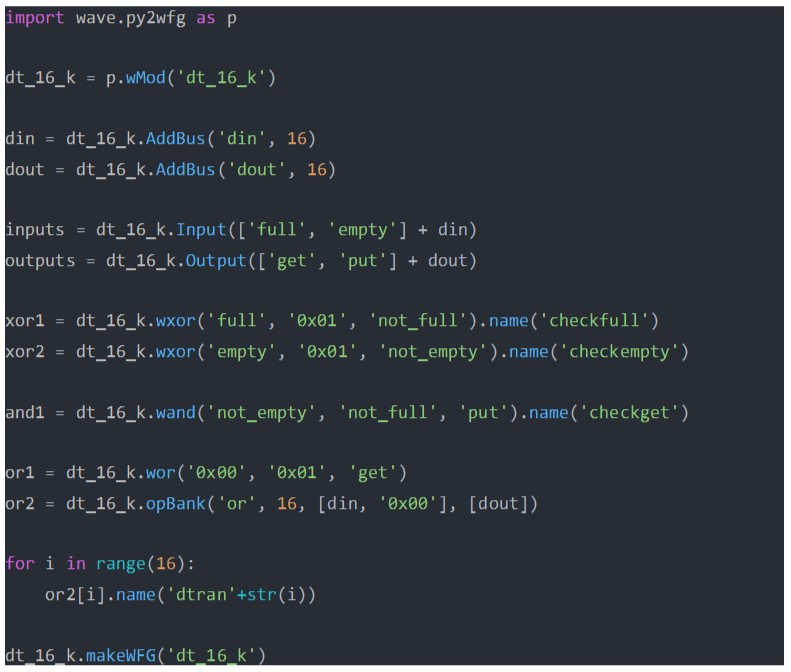
\includegraphics[trim=0cm 0cm 0cm 0cm, clip=true,scale=0.7]{figures/py2wfg_eg.jpg}
    \caption{Example Py2WFG script\label{Fig:py2eg}}\vspace{-4mm}
    \end{figure}

\paragraph{}
Running the example script shown in Figure~\ref{Fig:py2eg} will output a WFG file that contains the operations represented in the script, which is shown in Figure~\ref{Fig:wfgout}

\begin{figure}[h]
    \centering
    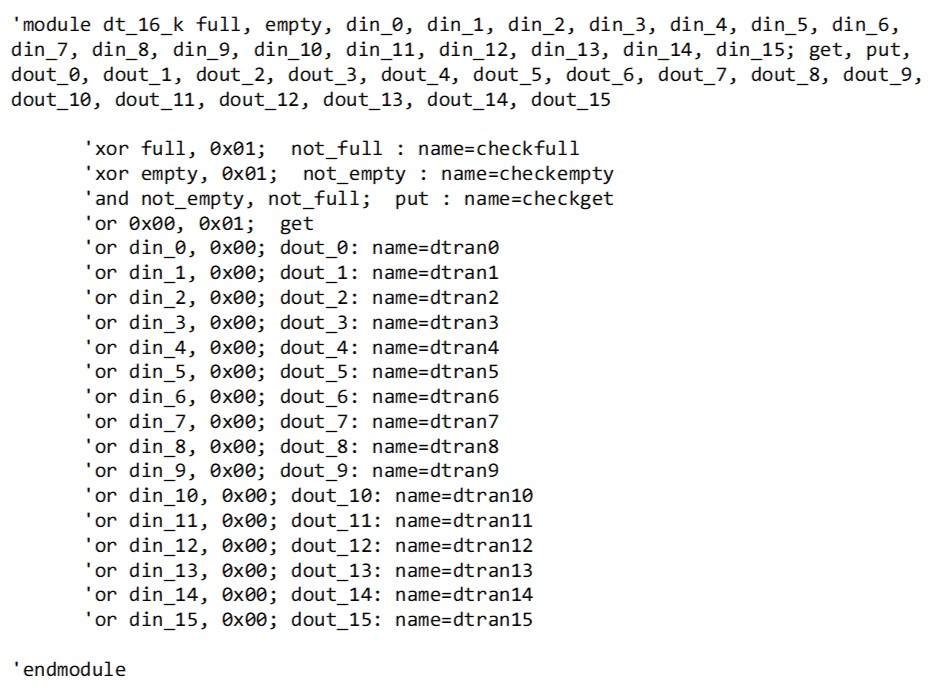
\includegraphics[trim=0cm 0cm 0cm 0cm, clip=true,scale=0.5]{figures/wfg_out.jpg}
    \caption{Output of the Py2WFG code from Figure~\ref{Fig:py2eg}\label{Fig:wfgout}}\vspace{-4mm}
    \end{figure}

\paragraph{}
This output WFG script unlike the handwritten scripts, is properly formatted and can be reconfigured easily through the python script again. This ease of use further improved with the introduction of the Simulator (section~\ref{sec:py2wfgsim}).

\subsubsection{Library Structure}
\subsubsection*{Data Types}
Main data types used in modeling a WFG module using Py2WFG are,
\begin{itemize}
    \item Primitive
    \item Pseudo
    \item Module
    \item Net
\end{itemize}

\subsubsection*{Primitive}
\paragraph{}
Primitives are basically WFG dataflow operations such as and, or, xfers, channel. These usually have inputs, outputs and attributes, depending on the specific primitive. These are the primary building blocks of a module.

\subsubsection*{Pseudo}
\paragraph{}
These are used for depicting memory operations such as ram and rom. They have connections different from dataflow operations but still have attributes just like dataflow.

\subsubsection*{Module}
\paragraph{}
Primitives and Memory get together to form modules. A module can correspond to a single WFG file or in more complex designs, several instances of one module can be created inside another module to form a hierarchical design.

\subsubsection*{Net}
\paragraph{}
These are somewhat similar to wires. They are used to interconnect modules and primitives. A collection of nets, grouped together for a common purpose is known as a bus.

\subsubsection{Python to WFG Simulator}
\label{sec:py2wfgsim}

\paragraph{}
The simulation of flow graph files are now done through WFGsim (section \ref{sec:wfgsim}). This platform is very complex and simulating a design on it takes a lot of overhead. To avoid this, an idea came up to add the ability to simulate Flow Graph designs on the Py2WFG library itself. This would allow the user to quickly write up a design on python and without exiting the python shell, they could quickly and efficiently simulate the design. 

\paragraph{}
Before calling up the simulator, if you need to test your designs against custom inputs, you need to define them in a special file called a input/output vector (iov) file.

\begin{figure}[h]
    \centering
    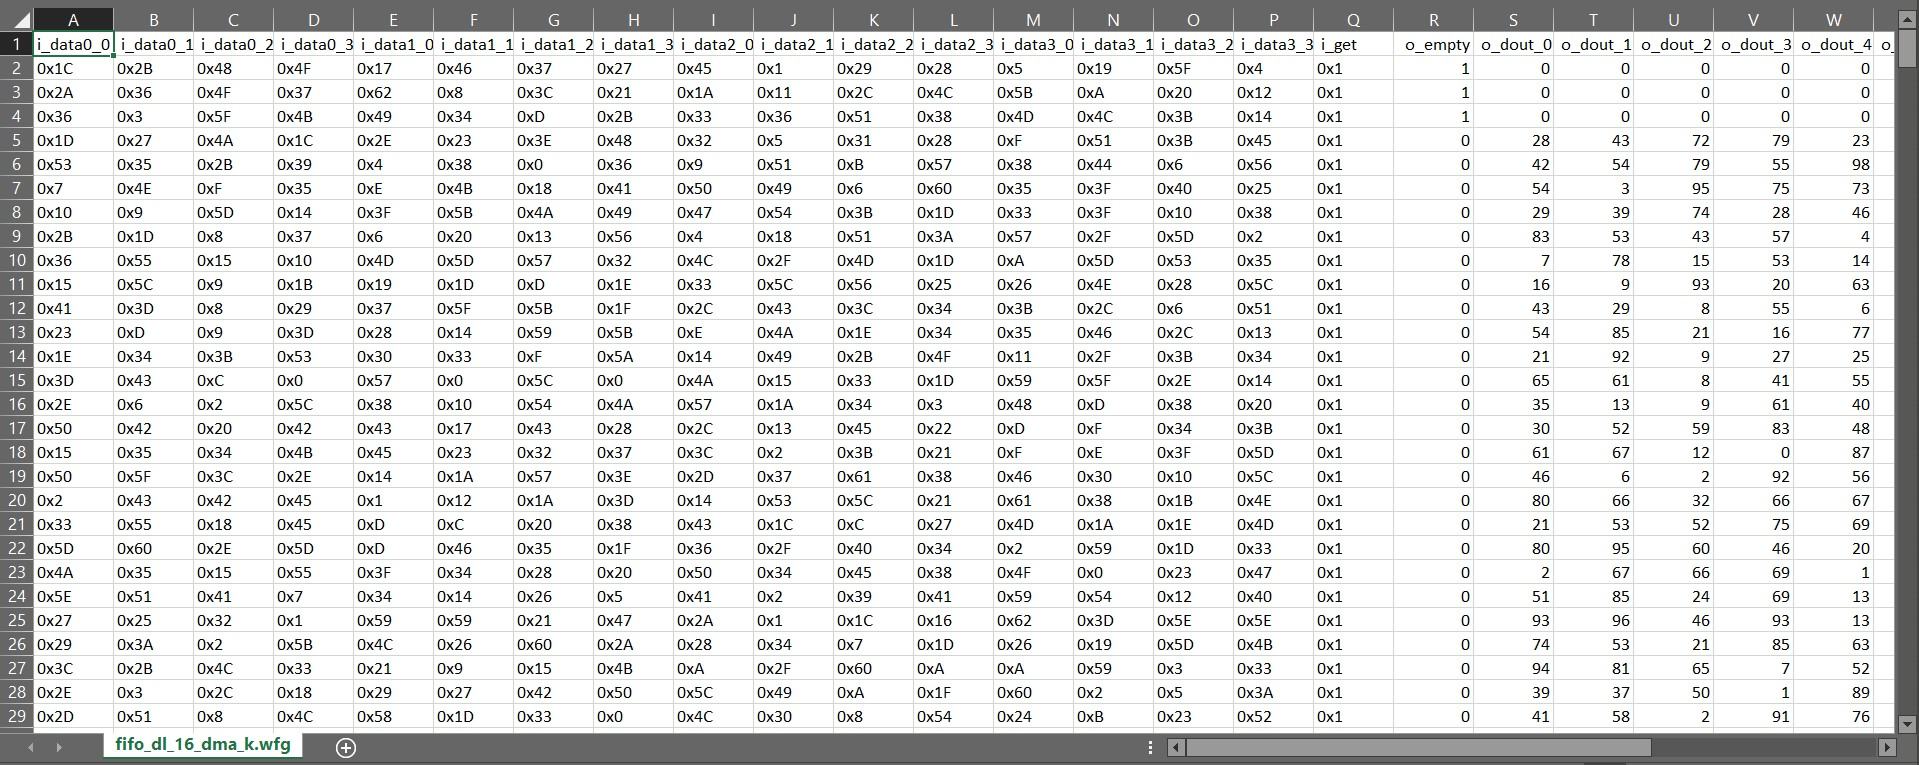
\includegraphics[trim=0cm 0cm 0cm 0cm, clip=true,scale=0.4]{figures/iov.jpg}
    \caption{A typical IOV file\label{Fig:iov}}\vspace{-4mm}
    \end{figure}

\paragraph{}
The values in Figure~\ref{Fig:iov} show the I/O values to and from the design in each tick the design was run for. The values that start as '0x' are input values, fed in hexadecimal format. Other values are the outputs which are in the decimal format. this is how WFGsim works, taking values in hexadecimalformat and outputting results in decimal. 

\paragraph{}
Py2WFGsim can accept values in any base but it is also configured to mimic the behavior of WFGsim by default. It will look for this iov file upon startup, and if found, will simulate the design with those inputs and if unable to find this file, will generate a user configurable number of random input vectors (1000 by default) and run the simulation on them. User also has the option to define expected outputs for a given set of inputs and test it against the actual outputs. This makes Py2WFGsim a strong verification tool.

\begin{figure}[h]
    \centering
    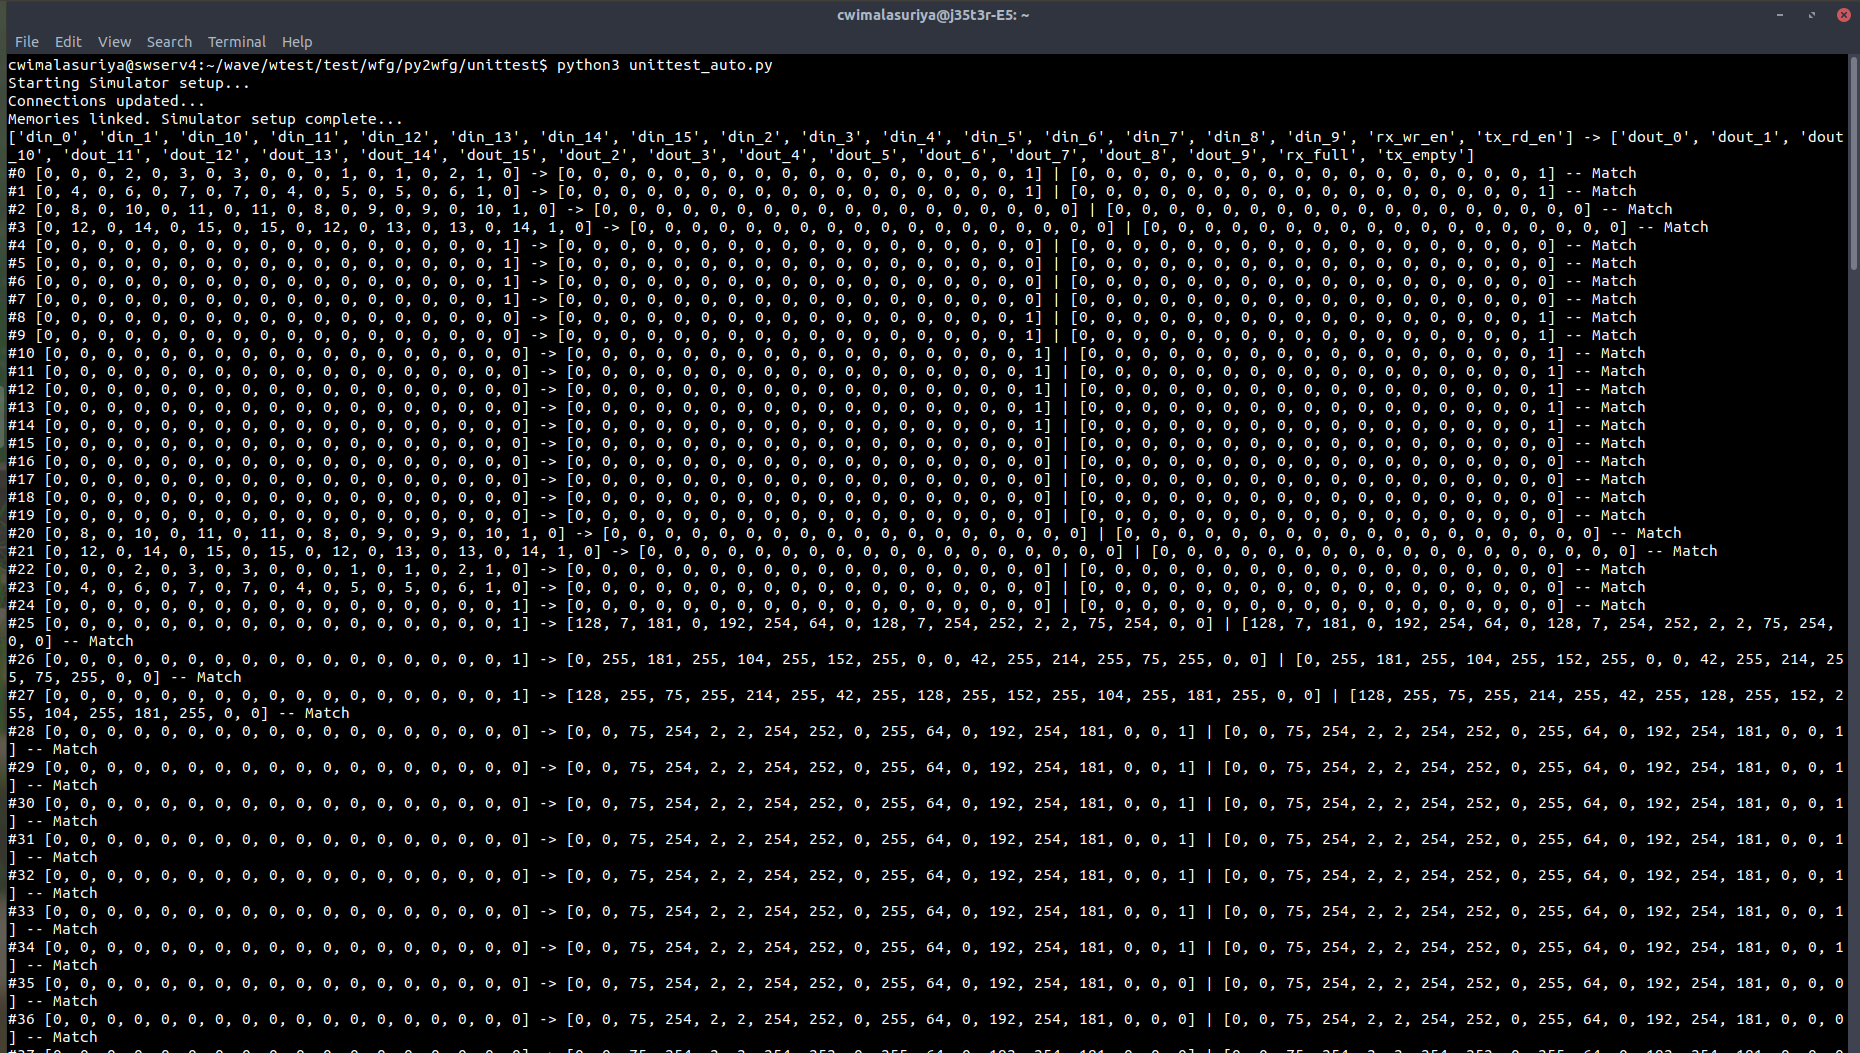
\includegraphics[trim=0cm 0cm 0cm 0cm, clip=true,scale=0.3]{figures/sim_result.png}
    \caption{Py2WFGsim user interface\label{Fig:simresult}}\vspace{-4mm}
    \end{figure}

\subsubsection{DMA engine}
\paragraph{}
The last part of the Project was implementing the DMA engine which was also the most controversial part since even now the engineers are having trouble with how this works. It is also known to slow down WFGsim and cause crashes and mismatches of all kind.

\begin{figure}[h]
    \centering
    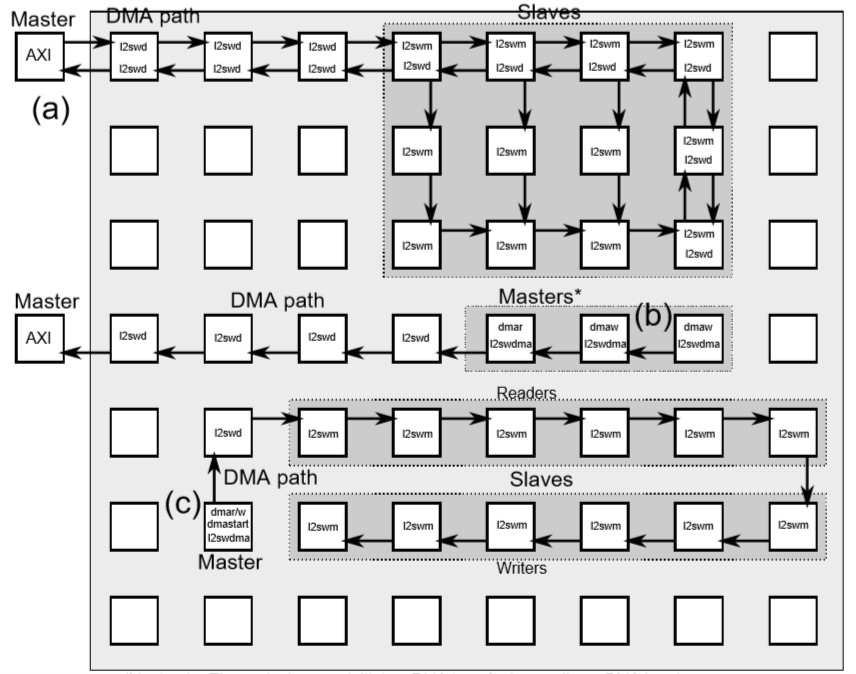
\includegraphics[trim=0cm 0cm 0cm 0cm, clip=true,scale=0.5]{figures/dma_path.jpg}
    \caption{Wave DPU DMA path\label{Fig:dmapath}}\vspace{-4mm}
    \end{figure}

\paragraph{}
DMA controller needs to be capable of communicating with an external host and managing the data transfers within the chip. These transfers are asynchronous and can occur at any time, making it highly challenging to implement it in a software based platform. Therefore, we decided that the DMA transactions and processing of data do not need to be executed in parallel for the time being. Another important decision is to altogether eliminate multi-thread programming, because it was identified as one of the major culprits of the poor performance in the original WFGsim. We opted for a linear implementation where only one operation executed at one time.

\paragraph{}
The final implementation consisted of standalone hosts that user can create and link to the channels of the design. Then the host would have R/W queues for each channel which it would properly execute as the time in the simulator passes by. This allows the user to freely schedule the host behavior without considering complex timing constraints. This design was successfully integrated to the simulator and it got accepted by the SDK team as a capable tool.

\subsubsection{Unit Testing}
\label{sec:unittest}

\subsubsection{International Testing}
\paragraph{}
To test out the translator/Simulator functionality, I was facilitated with a testing team consisting of people working from different countries including USA and China.

\begin{figure}[H]
    \centering
    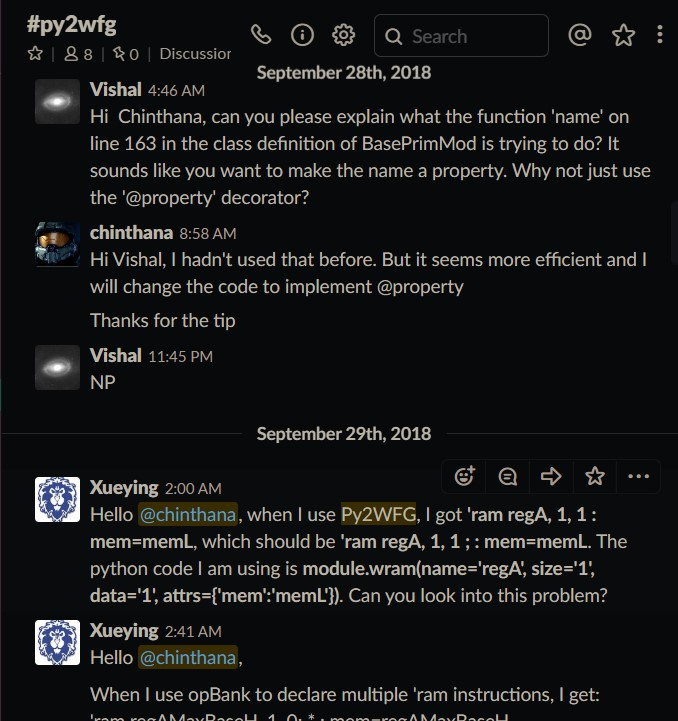
\includegraphics[trim=0cm 0cm 0cm 0cm, clip=true,scale=0.5]{figures/global_team.jpg}
    \caption{Communications with the overseas testing team\label{Fig:globalteam}}\vspace{-4mm}
    \end{figure}

\paragraph{}
This testing team was always helpful and efficiently reported whatever issues that the original designs had and came up with suggestions on best ways to solve the problems. They were a novel experience to me since I had never worked with a team scattered around the globe. It was rather efficient due to the software delivery system Wave has in place, allowing me to quickly deliver a fully tested builds of software to people in USA or China.
%!TEX root = ./intern_report.tex

\newpage
\subsection{Wave external software tools}
\subsubsection{Overview}
\paragraph{}
Working at Wave computing, I was exposed to the use of a lot of software automation tools that are used all over the world in design, development and testing of large scale industrial projects. Working with this expensive software with a crucial part of my internship experience.

The main external software tools used by wave are,
\begin{itemize}
    \item GitLab
    \item Jenkins
    \item Confluence
    \item Jira
    \item Slack
    \item Zoom
\end{itemize}

\paragraph{}
Apart from these software wave computing uses other special software in testing procedures. In general view, working with these expensive software tools is one of the best experiences that I obtained during the internship of six months.

\subsubsection{GitLab}
\paragraph{}
Wave computing uses GitLab as the main version control software. Since the use of version control in development of software project was not an entirely familiar topic for me I started working with them from scratch. I learnt about the efficient use of such systems and their various advantages in development of software projects. I realized the significance of such systems where developers from scattered everywhere could work according to a centralized plan and develop the same project from different operating from different parts of the world. Apart from that I experienced the advanced techniques used by large development communities in order to track every step of the development of a large scale project. 

\subsubsection{Jenkins}
\paragraph{}
Wave computing uses Jenkins as the test base for their automated testing procedure. Use of Jenkins in testing was an entirely new experience for me. A test run on Jenkins covered up all tests that are needed to be run on any wave flow graph design. After compilation and verification of the functionality of each wave flow graph design I was requested to run a mandatory test done on Jenkins before merging it with the main design of the master. In the event of failure of any of the designs I was assigned to investigate the reasons, rerun tests and make sure that the design was fully functional before engaging it with the main design. 

\subsubsection{Confluence}
\paragraph{}
Documentation of all Wave Computing related details are maintained in a Confluence page. I witnessed the importance of documentation while exploring various archives of Wave design development tools. I realized the downside to apparent dissatisfaction among the developers in maintaining properly updated archives of software development projects. I ran into a number of troubles due to outdated or insufficiently developed documents, specially about the DMA engine of the WFGsim. This contained a number of conflicted documents scattered around the Confluence site. However, I managed to gather these documents and extract a final definition of the DMA engine and build a replacement on my own.

\subsubsection{Jira}
\paragraph{}
Jira is the official issue tracker for Wave Computing team. Any issues, bugs, improvements or changes to the wave design flow are recorded as tasks in Jira. Resolving these tasks can be assigned to any of the design individuals of the wave computing team. Usually the tasks come with supervisors and senior consultants in charge of completion of it. Any changes or developments to that is updated to the Jira so that everyone can access the information and get an idea about the current status of the Wave design tools. It is a very convenient way of managing projects and deciding on the development of software project carried out with collaborators from all over the world. 

\subsubsection{Slack}
\paragraph{}
All the text based communication within Wave is carried out via Slack. It is like a normal instant messaging app that we have for our normal usage (Eg. Whatsapp) but has a lot of Enterprise focused features. It has the capability to separate work related content on channels, organize notifications on priority and enhanced search/organization capabilities. It is also available in almost every platform, mobile, windows, linux or web, making it perfect for a company that uses many platforms on their computing systems.

\subsubsection{Zoom}
While slack handles texting, zoom is the video calling platform of Wave. As the management of the company is overseas, high quality video calling is essential for Wave. Zoom provides this with their highly optimized VoIP technologies. Even when the internet connection is poor, which is a common problem in Sri Lanka, Zoom can maintain an acceptable link over it. 
%!TEX root = ./intern_report.tex

\newpage
\subsection{Life at CSIRO}

\paragraph{}
CSIRO, being a world class research institute, thrives to create a stress-free work environment that encourages people to socialize and to boost creativity. There is a workplace culture in DATA61 to bring cakes (or any equivalent sweets) for all the coworkers if one gets married, arrive at CSIRO, leave CSIRO, has a birthday and so on. I shared Sri Lankan sweets (sent by my mother in mail) for my birthday and cakes with everyone for arriving at and leaving CSIRO.

\subsubsection{Reading Groups and DATA61 Meetings}

\paragraph{}
Every friday, a small meeting called "Robotics Reading Group" is hosted, where one scientist explains his current project to everyone who attends the meeting. This way, we get to know the latest technology that is being developed in different parts of DATA61 and new projects that are being started. This meeting also allows the scientist to be questioned, so that he can derive insights from the audience and refine his procedures in the future. Also, once in a fortnight our supervisor Nick holds a "ML Robotics" meeting for all engineers working on machine learning. There we discuss our current ideas and issues to help each other. In addition to these, there are monthly meetings with the entire CSIRO (branches from all over Australia join via video conferencing), where new developments are discussed. One such meeting had the lead scientist from NASA's Insight Mars Lander mission as the chief guest explaining the challenges faced in their mission and taking our questions on the matter.

\begin{figure}[H]
    \centering
    
\includegraphics
        [width=12cm]
        {figures/presentation.png}
    \caption{Presenting the Pipeline in Robotics Reading Group}\vspace{-4mm}
\end{figure}

\subsubsection{Presenting the Pipeline at Reading Group to the Scientists}

Uvindu and I presented the pipeline to other scientists during one of the last Reading Group meetings of the year. It was well received, thanks to the support of our supervisor who encouraged others to use our pipeline in their workflow. Many asked questions and were convinced of the merits of such a unified framework. I had a few scientists reaching out to me on the following days asking me to develop visualization tools to complement the pipeline. 

\subsubsection{DATA61 Live Event}

DATA61 Live is an event held annually to showcase the science and technology innovations of DATA61 from all over Australia. In 2018, it was held in Brisbane, in our city. The theme was: 'Adapting to Disruption'. We signed up as volunteers and apart from volunteering, we had a chance to attend many lectures, talks and forums. It was a great experience.

\begin{figure}[H]
    \centering
    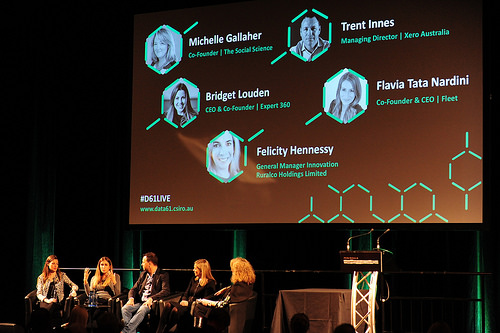
\includegraphics
        [height=5cm]
        {figures/data61_live_1.jpg}
    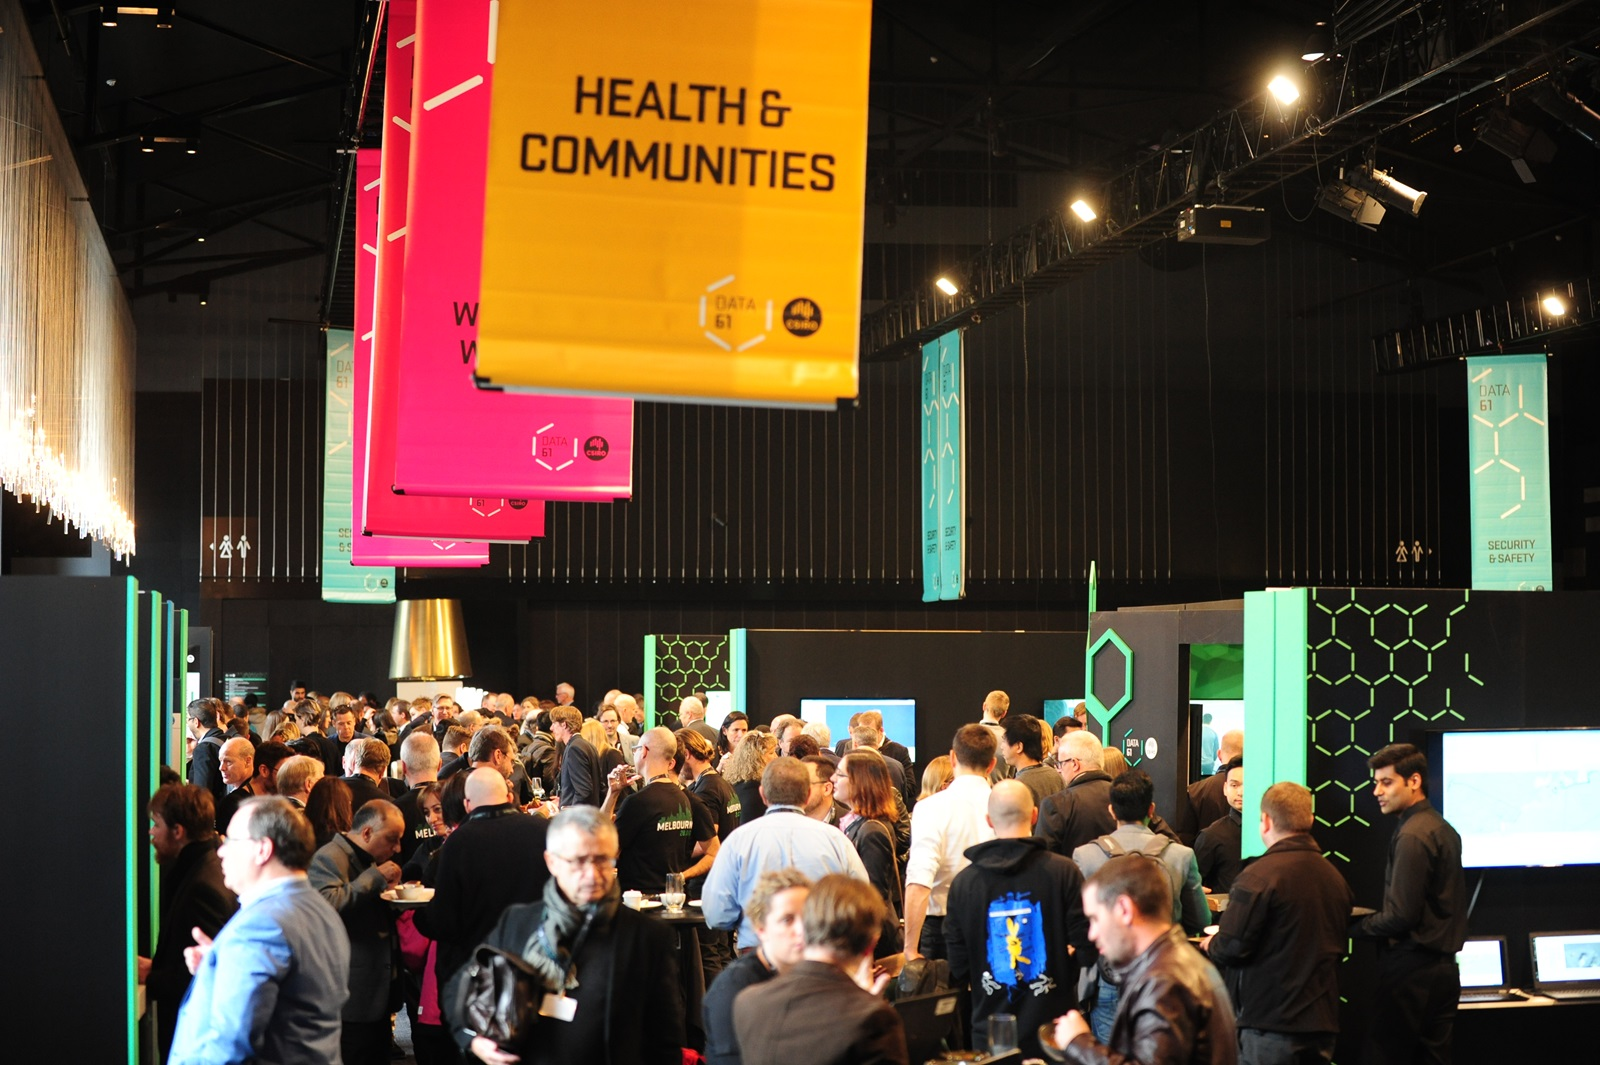
\includegraphics
        [height=5cm]
        {figures/data61_live_2.jpg}
    \caption{DATA61 LIVE Event}\vspace{-4mm}
\end{figure}

\newpage
\section{Conclusion}
%!TEX root = ./intern_report.tex

\paragraph{}
I worked as a research intern at DATA61 for 24 weeks. During this time, I worked three intertwined projects under the supervision of Nicolas Hudson and Dr. Navinda Kottege. 

\paragraph{}
The first project was developing indoor-Trailnet: a classification based approach to the autonomous navigation problem. For this, first I built a robot with Uvindu Perera for data collection and testing. We designed the power distribution system of the robot and assembled a high level and low level controllers. We calculated the torque requirements for the motors, current, voltage and power limitations for the power supply components and motor controllers during this process. We learnt a lot through debugging the errors we came across and extensively troubleshooting whenever a component or circuit board is damaged to provide a report on the event. I also debugged the driver software for the motor controller and modified parts of it to fix certain issues since it was not being maintained anymore.

\begin{figure}[H]
    \centering
    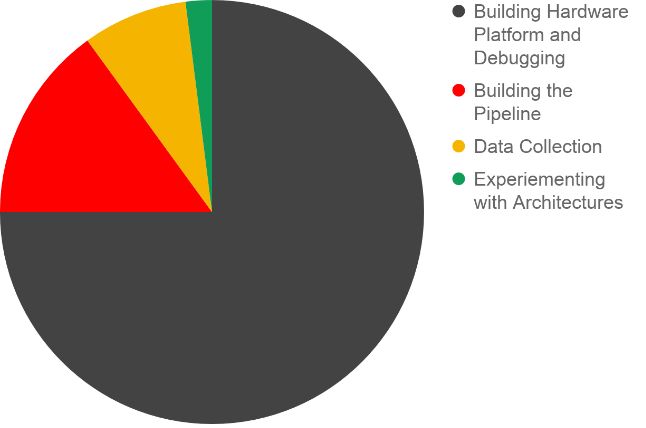
\includegraphics
        [width=9cm]
        {figures/time.PNG}
    \caption{Overview of our Time Spent}\vspace{-4mm}
\end{figure}

\paragraph{}
I learnt tensorflow and tensorflow-keras for this project and built a 20 layer residual network from scratch and trained it on the supercomputer cluster. Then I learnt tensorRT and deployed the trained network on Jetson TX2: a powerful embedded device that acted as the high level controller for the robot. I also learnt ROS (Robot Operating System) extensively, and created multiple ROS nodes and packages for testing, collecting data from sensors and for controlling the robot. 

\paragraph{}
For the next project of building an end to end pipeline for machine learning in robotics, I experimented and figured out the best practices when training models using large datasets on the supercomputer. I documented these experiments and the results, and proposed an efficient method to set up a writing and reading pipeline. I presented ~\cite{presentation} my pipeline in the Robotics Reading Group meeting. Many scientists were interested and some followed up via email asking questions and requesting to build tools for visualizing datasets.

\paragraph{}
The final project was experimental, where I explored different configurations of neural network architectures to build a robot that can climb hills while avoiding obstacles. Through literature survey and in-depth discussions with my supervisor, I learnt a lot about the structure of Deep Convolutional Neural Networks and possible methods of combining scaler data with the images to train a network. I tried several approaches here: solving the problem as a classification and a regression and using different ways to combine the inputs into the network. However, I was unable to get good results within the time we had there, due to the problems in data collection and the lack of time as we had to spend most of the time building and debugging the robot platform.

\paragraph{}
Also, I learnt about cross modal learning transfer and neural network distillation process through literature survey as a part of the project that was initially given, before we were changed into a different project a week later. Before and during the internship program, I expressed my interest in working in a project where I can develop algorithms and tackle abstract problems that could lead to new research and a publication. Unfortunately such a project was not available for interns at the time and my supervisors were satisfied with the work I was doing with hardware and deployment of machine learning. However, I learnt a lot through these projects and it had been a great experience. I also got familiarized with the software tools widely used in academia, high end sensors and controllers, and I daily worked with the Bracewell cluster, which is one of the world's largest supercomputer clusters. 

\paragraph{}
In addition to that, I learnt the etiquettes and responsibilities of working as an employee in a company. Helping others and asking for help, attending meetings and following up via official emails, documenting all the tasks and weekly progress in the wiki pages of CSIRO helped me learn a lot about these responsibilities. The work culture in DATA61 is exceptionally inclusive, where we got to work with people of multiple nationalities and share our culture. The students are allowed to work on their own pace and I was allowed to work overnight on multiple days and work on weekends as well. I also got to attend events such as DATA61 LIVE, where I could attend to many talks and discussion forums and observe the development of cutting edge technology of Australia through the exhibits.

\paragraph{}
From my experience, I would suggest DATA61 to assess the skills of the interns and assign them to projects relevant to those skills, to utilize their full potential for a project. Also, it would help if they can give an overview of the project at the beginning of the internship and set incremental goals to be completed at given deadlines. I found it disorienting when the project given to me before the internship was changed as I reached there and changed again a week later to settle on an experimental project of my supervisor that subsequently evolved into the three above projects (that I explained in Chapter 2) through the period of six months. 

\paragraph{}
I would also like to suggest NAITA to computerize the supervision process, where interns can submit the intern diary and monthly reports online. This would help because in organizations like CSIRO, the students are expected to maintain an online diary and the interns can save time by writing by hand the same thing they have typed into the online diary.

\paragraph{}
Therefore, I can conclude that my overall experience in DATA61 was great. I had the opportunity to learn a lot and make contacts. I am deeply thankful to the Industrial Training Division of our university and NAITA for this internship and I am thankful for DATA61 and my supervisors for providing me with such an exceptional opportunity and a training experience.







\newpage



\bibliographystyle{abbrv} 
\bibliography{biblo}
\end{document}